\documentclass[conference,letterpaper]{IEEEtran}
\usepackage[T1]{fontenc}
\usepackage[utf8]{inputenc}
\usepackage{cite,graphicx,xurl,microtype}
\usepackage[hidelinks]{hyperref}
\title{Encore Moment\\[0.3em]
{\large Audience Reaction Capture for Smart TVs}\\[0.4em]
{\normalsize Group Encore}}
\author{
\IEEEauthorblockN{Chul Park}
\IEEEauthorblockA{Department of\\Information Systems\\
Hanyang University\\Seoul, Republic of Korea\\parkchul1@hanyang.ac.kr}
\and
\IEEEauthorblockN{Pavel Kim}
\IEEEauthorblockA{Department of\\Information Systems\\
Hanyang University\\Seoul, Republic of Korea\\skydish@hanyang.ac.kr}
\and
\IEEEauthorblockN{Soyeon Seol}
\IEEEauthorblockA{Department of\\Information Systems\\
Hanyang University\\Seoul, Republic of Korea\\ssy050915@hanyang.ac.kr}
\and
\IEEEauthorblockN{Yujeong Heo}
\IEEEauthorblockA{Department of\\Information Systems\\
Hanyang University\\Seoul, Republic of Korea\\gjdbwjd03@hanyang.ac.kr}}
\hypersetup{pdftitle={Encore Moment - Submission A: Proposal and Requirements},
pdfauthor={Group Encore},pdfsubject={CSE406 Software Engineering - Submission A}}
\begin{document}
\maketitle
\begin{abstract}
Encore Moment is a proposed smart TV service for preserving spontaneous audience reactions as personal viewing memories. Friends, couples, families, party guests, and streamers may wish to revisit a shared laugh or surprise without interrupting the experience to record it. The service will recognize laughter, screams, and gasps, associate them with content titles and timecodes, and offer a live timeline and post-viewing highlights. Optional audience video will remain under explicit user control. This proposal defines stakeholder needs, reviews relevant models, datasets and capture software, and presents team responsibilities and requirements. The scope includes server-based analysis and Kubernetes deployment, subject to verification of the required TV interfaces.
\end{abstract}
\begin{IEEEkeywords}
smart TV, audience reactions, shared viewing, sound event detection, reaction clips, requirements analysis
\end{IEEEkeywords}
\section{Introduction}

\subsection{Motivation}

A memorable viewing experience includes the people in the room. Friends may laugh at the same unexpected line, a couple may gasp at a plot twist, or a home party may erupt during a tense scene. These reactions can carry the mood of the occasion more vividly than a photograph taken afterward. They also happen without warning. Reaching for a phone after the moment has passed cannot recover the initial reaction, while recording an entire evening leaves users with material to search and edit.

We propose Encore Moment to help viewers preserve these spontaneous moments while remaining engaged with one another and the screen. Research on preserving everyday laughter describes both the enjoyment of revisiting it with loved ones and the tensions involved in collecting it \cite{ref1}. This supports treating reactions as personal memories, while leaving users in control of what is retained. It does not establish demand for a TV service; the viewing scenarios in this proposal are intended use cases to be validated with users.

\subsection{Target Users and Viewing Contexts}

Friends watching together and guests at a home party may want a short record of the group's response without assigning someone to act as a camera operator. Couples on a movie date may value a shared expression or quiet moment of surprise, making unobtrusive operation and clear recording choices especially important. Families may wish to revisit reactions across ordinary evenings as well as special occasions. Across these settings, the value lies in who was present and what happened together, rather than simply accumulating recordings.

Streamers and reaction-content creators form an additional audience. They may need to find spontaneous reactions after a viewing session without reviewing the entire recording. Their editing needs differ from private social viewing, but both groups benefit from useful event markers and reviewable clips. Encore Moment focuses on finding and preserving candidate moments; users decide whether a saved moment is suitable to keep or use elsewhere.

\subsection{User and Client Needs}

Viewers need relevant highlights, enough context to remember the scene, and controls that are easy to understand during viewing. A film's laugh track or scream should not be mistaken for a person in the room. Users should know when sensing is active, be able to stop it, and review or delete saved clips. Reaction intensity can help prioritize review, but it cannot determine a person's emotional state or the personal importance of a memory.

For this proposal, the assumed client is a smart TV service provider seeking a useful viewing feature that fits an existing TV experience. LG smart TV integration is the intended project context. The client needs a clear feature scope, understandable privacy controls, and honest statements about supported devices and content access. These are proposed client needs, not confirmed contractual requirements or completed interview findings.

\section{Related Software}

This preliminary review compares existing products, candidate models, datasets, and capture interfaces. It identifies relevant capabilities and unresolved dependencies before model selection and device testing.

\subsection{Existing Capture and Highlight Services}

SteelSeries Moments introduced microphone-triggered clipping for laughter and excited vocal reactions \cite{ref2}, later naming the feature Reaction Clipping \cite{ref3}. This is a close precedent for Encore Moment's event-triggered capture. Twitch Auto Clips describes automatic clip creation through speech recognition and artificial intelligence (AI); its documentation currently presents an invitation-only, English-language alpha \cite{ref4}. Reaction-triggered and automatic clipping are therefore established approaches in gaming and streaming software.

Medal provides event-triggered clipping through integration with a game \cite{ref5}. OBS Studio exposes controls to start, stop, and save a replay buffer \cite{ref6}, making recent-moment capture accessible to recording workflows. These examples inform the relationship between an event and its saved media. Encore Moment's proposed emphasis is the shared TV viewing context: distinguish audience reactions from playback sound, retain the associated scene context, and let participants control their personal recordings.

\subsection{Sound Event Models}

YAMNet, available through Google's Kaggle model page, is a candidate baseline for environmental sound classification \cite{ref7}. Its class vocabulary includes laughter, screaming, and gasp. TensorFlow provides a transfer-learning example that uses YAMNet embeddings for a new classifier \cite{ref8}. This makes it a practical starting point for examining the required categories and nearby confusions such as speech or breathing. The existence of those labels does not establish accuracy for distant or overlapping audience reactions.

The Audio Spectrogram Transformer (AST) checkpoint hosted by MIT on Hugging Face offers an AudioSet-trained comparison and also includes the three target categories \cite{ref9}. Pretrained Audio Neural Networks (PANNs) provide both clip-level tagging and sound-event variants with framewise outputs \cite{ref10}. That distinction matters for the proposed timeline: identifying a sound somewhere in a clip does not necessarily locate its beginning and end. We therefore consider YAMNet and AST as classification candidates and the PANNs sound-event variant as a temporal-detection reference.

Additional candidates address different questions. EfficientAT provides efficient audio-tagging models suitable for later comparison of resource use and recognition quality \cite{ref11}. Microsoft BEATs supplies pretrained audio representations as well as classification checkpoints \cite{ref12}. LAION CLAP relates audio to textual descriptions and can support exploratory zero-shot comparisons \cite{ref13}. These are secondary options rather than simultaneous dependencies; a feature encoder, a class prediction, and an audio-text similarity score are different outputs.

Speech-emotion models require a separate justification. For example, audEERING's dimensional emotion model was trained on English podcast speech and predicts arousal, dominance, and valence; its model card also specifies research-use restrictions \cite{ref14}. That task differs from identifying brief nonverbal reactions. The present proposal therefore focuses on observable sound categories. Classifier confidence, acoustic intensity, and subjective emotional significance will not be treated as interchangeable measures.

\subsection{Datasets and Evaluation Relevance}

FSD50K is a strong data candidate because it provides human-labeled audio, including laughter, screaming, and gasp \cite{ref15}. Its clip-level labels do not directly provide precise reaction boundaries or intensity annotations, and individual sound licenses must be checked. FSDKaggle2019 provides additional curated and noisy audio-tagging data \cite{ref16}. Its official class map includes gasp and screaming but no laughter class \cite{ref17}, so it cannot alone cover all three required reactions.

FSD50K incorporates much of the human-labeled FSDKaggle2019 material \cite{ref15}. The two collections must therefore not be treated as independent training and evaluation sets without checking overlap. VocalSound offers complementary examples of laughter, sighs, coughs, throat clearing, sneezes, and sniffs \cite{ref18}. It is useful for studying confusing human sounds, but does not contain the required gasp and scream categories.

Public recordings can support initial model comparisons, but the intended environment introduces additional questions: whether TV dialogue causes false detections, whether quiet reactions remain detectable, and how simultaneous voices or room reverberation affect results. Later validation should include consented viewing recordings, soundtrack-only cases, and mixed audience/playback sound.

\subsection{Echo Cancellation and Audio Processing}

Acoustic echo cancellation (AEC) is relevant because a classifier can correctly recognize laughter that actually originates from the TV. WebRTC's Audio Processing Module provides playback-reference and microphone processing interfaces relevant to AEC \cite{ref19}. The Microsoft AEC Challenge supplies data, baselines, and evaluation resources for echo research \cite{ref20}. Their use in speech applications does not establish that every nonverbal reaction will be preserved. Suppressing playback and retaining useful audience sound are both requirements, and depend on obtaining suitable input signals.

\subsection{Replay Buffers and Event Recording}

OBS Replay Buffer illustrates saving a recent interval after an interesting event \cite{ref6}. NVIDIA DeepStream Smart Video Record similarly supports event-triggered recording from cached media, including material before the event; its documentation notes keyframe-related limits on the available beginning of a clip \cite{ref21}. GStreamer splitmuxsink provides media-file segmentation and a limit on retained files \cite{ref22}. These are useful references for recent-moment storage, although none determines which audience reaction deserves a highlight. Camera control also limits what can be retained: a pre-event video segment can exist only if the camera was already enabled during that interval.

\subsection{TV and Capture Interfaces}

LG Smart Cam provides camera and microphone hardware for supported LG TVs \cite{ref23}, but device availability does not establish access from an ordinary application. A July 2026 LG developer-forum response states that no public application programming interface (API) retrieves media from a connected camera and that WebRTC access is restricted to contracted partner apps \cite{ref24}. The published webOS Audio API describes volume control rather than access to raw playback audio \cite{ref25}. Access to camera media, microphone audio, playback reference, titles, and timecodes must therefore be verified for the actual device and content source; universal compatibility with streaming applications is not assumed.

ReSpeaker XVF3800 is a development-input candidate with a microphone array and configurable audio processing \cite{ref26}. Its documented desktop-host support is not evidence of webOS compatibility. Such hardware is relevant to preliminary feasibility research, while the final interface choice remains open. Overall, the review supports investigation of the proposed features but identifies TV signal access and reaction-specific validation as conditions that must be resolved before broad compatibility claims.

\section{Team Responsibilities}

Table~\ref{tab:roles} assigns development roles and module ownership; SW denotes software. Soyeon Seol additionally represents the course User role, and Pavel Kim the Customer role. These internal stakeholder roles support review of proposed needs. All members participate in requirement reviews and integration checks.

\begin{table}[!ht]
\centering
\caption{Module Ownership and Role Assignments}
\label{tab:roles}
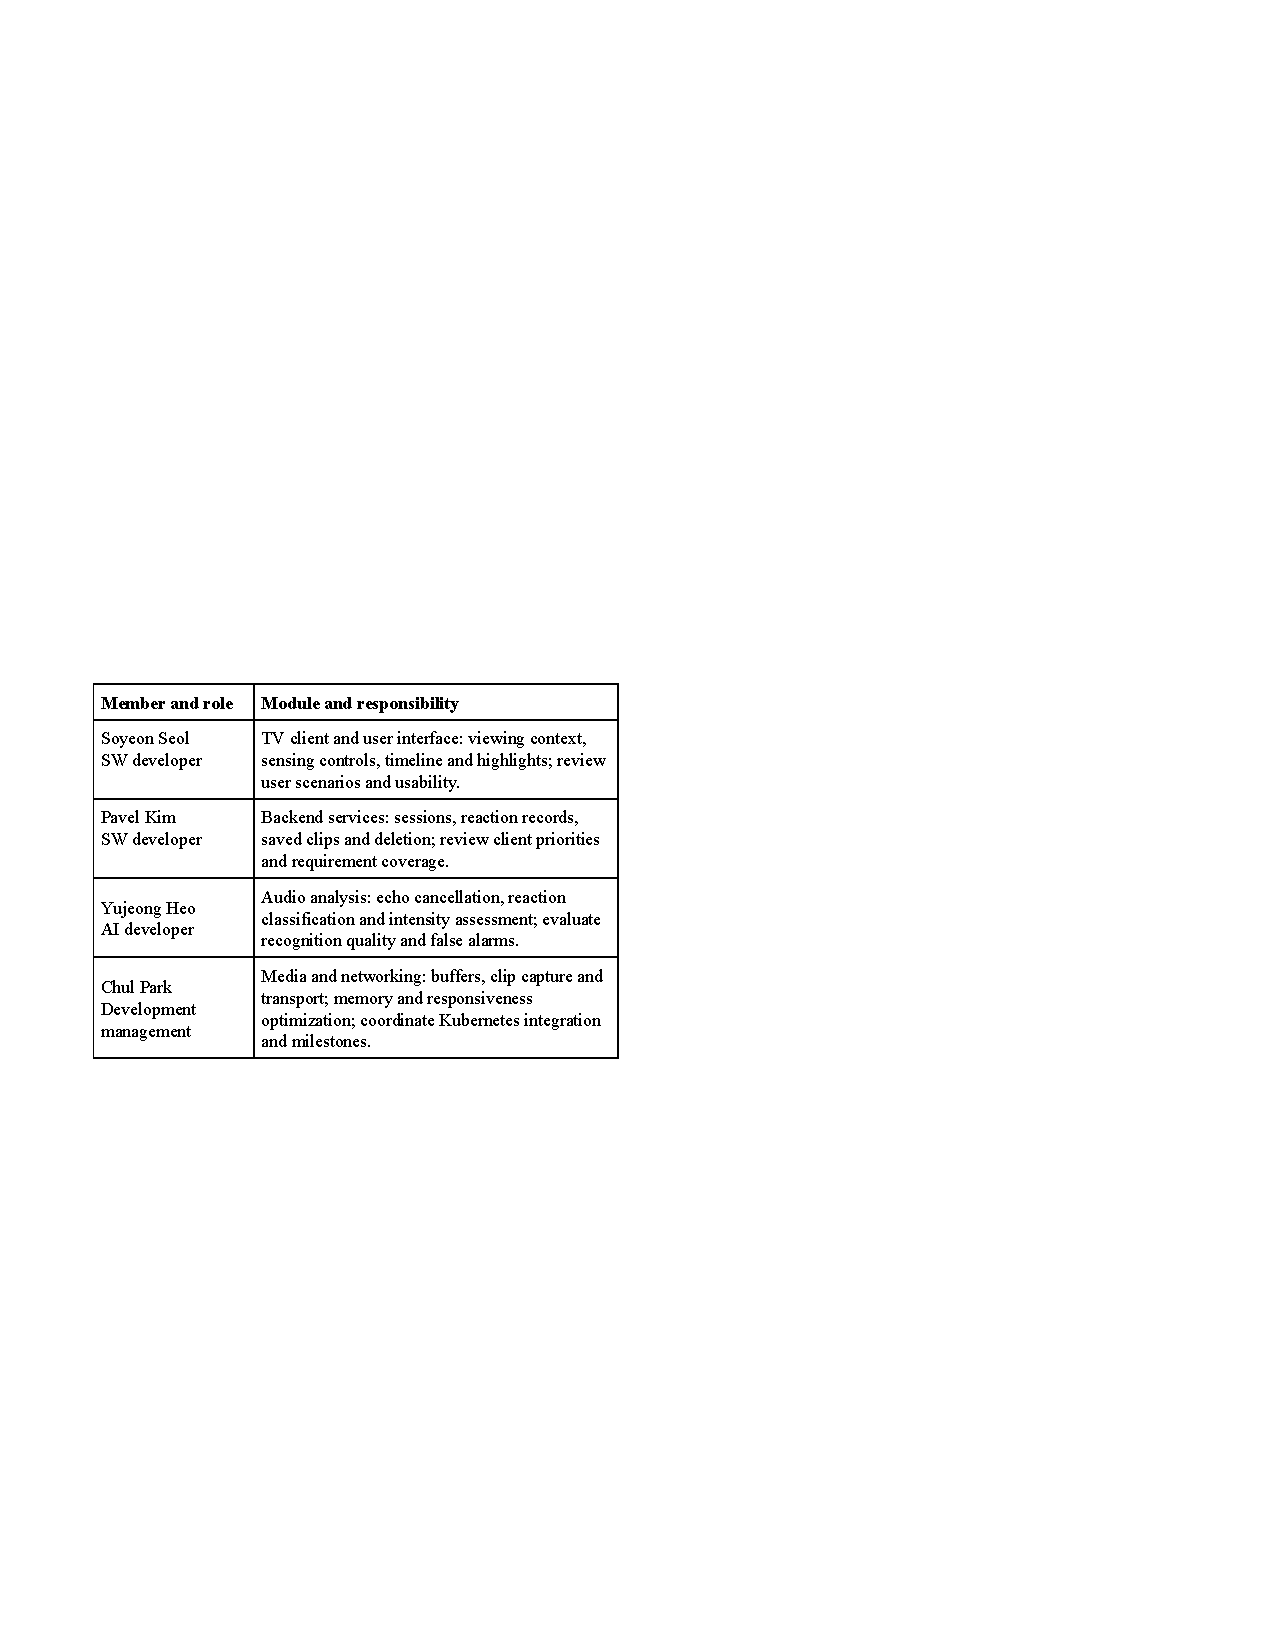
\includegraphics[width=\columnwidth]{images/team-roles.pdf}
\end{table}

\section{Requirements}

The following requirements define the viewing workflow and sensor controls. EIR identifies external interfaces, FR functions, PR qualitative quality objectives, and NFR privacy or operational constraints. Saved video refers to audience footage. Input-dependent features apply to supported, authorized sources, with unavailable capabilities disclosed to the user.

\subsection{External Interface Requirements}

\textbf{EIR-1 Room audio.} The system shall capture room audio from a supported TV or soundbar microphone. An equivalent development input may support initial testing; its use shall not imply native TV compatibility.

\textbf{EIR-2 Playback reference.} The system shall obtain the playback audio signal as a reference for echo cancellation. When the reference is unavailable, the system shall indicate that echo cancellation is unavailable.

\textbf{EIR-3 Viewing context and connection.} The TV client shall exchange viewing inputs and reaction results with the server, including content title, playback position, and playback-state changes needed to associate reactions with scenes.

\subsection{Functional Requirements}

\textbf{FR-1 Echo cancellation.} The system shall use the playback reference to suppress playback sound in microphone audio while retaining audience sound for reaction analysis.

\textbf{FR-2 Reaction recognition.} The system shall classify detected audience sounds into at least laughter, scream, and gasp.

\textbf{FR-3 Event records.} The system shall record each detected reaction with its type, observed intensity, content title, and timecode. Intensity shall describe the observable reaction rather than an inferred internal emotion.

\textbf{FR-4 Highlights.} After viewing, the system shall present Tonight's Highlights, prioritizing high-intensity reaction segments and linking any available audience clips for user review.

\textbf{FR-5 Camera activation.} The camera shall be off by default and activated only by explicit user action. No video shall be captured, buffered, or uploaded while it is off.

\textbf{FR-6 Camera indication.} The interface shall show a persistent indicator while the camera is active and provide a control to stop capture.

\textbf{FR-7 Review and deletion.} Users shall be able to review and delete saved reaction clips and their associated media at any time. The interface shall indicate whether a deletion request is pending or completed.

\textbf{FR-8 Microphone control.} Users shall be able to disable microphone-based sensing. This shall stop audio capture, upload, and new audio-triggered detections, with the disabled state shown clearly.

\textbf{FR-9 Viewing interface.} The interface shall display a real-time reaction timeline, the highlight list, and the current sensing and connection status.

\textbf{FR-10 AEC control.} The system shall provide an option to turn echo cancellation on and off and show the selected mode.

\textbf{FR-11 Reaction clips.} With the camera enabled, the system shall save audience clips containing available moments before and after a detected reaction. Missing portions shall be indicated; no footage from before camera activation shall be assumed to exist.

\textbf{FR-12 Viewing sessions.} Users shall be able to start and end sensing sessions. The system shall report connection interruptions, avoid duplicate reaction records after reconnection, and clear unsaved temporary media when a session ends.

\subsection{Qualitative Quality Objectives}

\textbf{PR-1 Reaction preservation.} Echo processing shall be developed to reduce playback interference while preserving audience reactions needed for recognition.

\textbf{PR-2 Non-reaction rejection.} The classifier shall handle ordinary speech, household noise, and uncertain sounds so that these are not automatically accepted as audience reactions.

\textbf{PR-3 False-alarm control.} The system shall support comparison of AEC-on and AEC-off detection to identify and reduce reactions falsely attributed to the audience when only the soundtrack is playing.

\textbf{PR-4 Responsive processing.} The system shall support reaction analysis and timeline updates during viewing, with clip saving able to proceed without blocking new detections.

\subsection{Privacy and Operational Constraints}

\textbf{NFR-1 Consent and access.} Users shall be informed of server processing before sensing begins. Camera activation shall require separate permission. Saved media shall be restricted to authorized users, and media transfers shall be authenticated and encrypted.

\textbf{NFR-2 Temporary media.} Continuous media shall be retained only in bounded temporary storage; selected clips and event metadata may be saved. Disabling a sensor shall clear its unsaved queued media.

\textbf{NFR-3 Server deployment.} The team shall provide server-based AI and computational processing, with the server components deployable on Kubernetes, a platform for managing containerized workloads and services \cite{ref27}.

Requirement checks will cover the viewing workflow, reaction records, AEC mode comparison, sensor controls, clip availability, and deletion. Public data and consented room recordings will support qualitative assessment under soundtrack-only, audience-only, and mixed conditions. Numerical performance targets are not specified in this proposal.

\IEEEtriggeratref{4}
\begin{thebibliography}{27}

\bibitem{ref1}
K. Ryokai, E. Durán López, N. Howell, J. Gillick, and D. Bamman, ``Capturing, representing, and interacting with laughter,'' in Proc. CHI, 2018, Paper 358, pp. 1--12, doi: 10.1145/3173574.3173932. [Online]. Available: \url{https://doi.org/10.1145/3173574.3173932}. Accessed: Oct. 22, 2026.

\bibitem{ref2}
SteelSeries, ``GG Release Notes 55.0.0,'' Jan. 23, 2024. [Online]. Available: \url{https://techblog.steelseries.com/2024/01/23/GG-notes-55.0.0.html}. Accessed: Oct. 22, 2026.

\bibitem{ref3}
SteelSeries, ``GG Release Notes 70.0.0,'' Sep. 4, 2024. [Online]. Available: \url{https://techblog.steelseries.com/2024/09/04/GG-notes-70.0.0.html}. Accessed: Oct. 22, 2026.

\bibitem{ref4}
Twitch, ``Auto Clips,'' Twitch Help. [Online]. Available: \url{https://help.twitch.tv/s/article/auto-clips}. Accessed: Oct. 22, 2026.

\bibitem{ref5}
Medal, ``Auto Clipping,'' developer documentation. [Online]. Available: \url{https://medal.tv/portal/docs/auto-clipping}. Accessed: Oct. 22, 2026.

\bibitem{ref6}
OBS Project, ``Frontend API,'' OBS Studio documentation. [Online]. Available: \url{https://docs.obsproject.com/reference-frontend-api}. Accessed: Oct. 22, 2026.

\bibitem{ref7}
Google, ``YAMNet,'' TensorFlow 2 model, ver. 1, Kaggle. [Online]. Available: \url{https://www.kaggle.com/models/google/yamnet/tensorFlow2/yamnet/1}. Accessed: Oct. 22, 2026.

\bibitem{ref8}
TensorFlow, ``Transfer learning with YAMNet for environmental sound classification.'' [Online]. Available: \url{https://www.tensorflow.org/tutorials/audio/transfer_learning_audio}. Accessed: Oct. 22, 2026.

\bibitem{ref9}
MIT, ``AST fine-tuned on AudioSet,'' model card and configuration, Hugging Face. [Online]. Available: \url{https://huggingface.co/MIT/ast-finetuned-audioset-10-10-0.4593}. Accessed: Oct. 22, 2026.

\bibitem{ref10}
Q. Kong, ``PANNs inference,'' source repository. [Online]. Available: \url{https://github.com/qiuqiangkong/panns_inference}. Accessed: Oct. 22, 2026.

\bibitem{ref11}
F. Schmid, ``EfficientAT,'' source repository. [Online]. Available: \url{https://github.com/fschmid56/EfficientAT}. Accessed: Oct. 22, 2026.

\bibitem{ref12}
Microsoft, ``BEATs,'' UniLM source repository. [Online]. Available: \url{https://github.com/microsoft/unilm/tree/master/beats}. Accessed: Oct. 22, 2026.

\bibitem{ref13}
LAION, ``CLAP HTSAT unfused,'' model card, Hugging Face. [Online]. Available: \url{https://huggingface.co/laion/clap-htsat-unfused}. Accessed: Oct. 22, 2026.

\bibitem{ref14}
audEERING, ``Wav2vec2 large robust 12 ft emotion msp dim,'' model card, Hugging Face. [Online]. Available: \url{https://huggingface.co/audeering/wav2vec2-large-robust-12-ft-emotion-msp-dim}. Accessed: Oct. 22, 2026.

\bibitem{ref15}
E. Fonseca, X. Favory, J. Pons, F. Font, and X. Serra, ``FSD50K: An open dataset of human-labeled sound events,'' arXiv:2010.00475, ver. 2, 2022. [Online]. Available: \url{https://arxiv.org/abs/2010.00475}. Accessed: Oct. 22, 2026.

\bibitem{ref16}
Freesound, ``Freesound Audio Tagging 2019,'' Kaggle competition. [Online]. Available: \url{https://www.kaggle.com/competitions/freesound-audio-tagging-2019}. Accessed: Oct. 22, 2026.

\bibitem{ref17}
DCASE, ``DCASE 2019 Task 2 baseline class map,'' source repository. [Online]. Available: \url{https://github.com/DCASE-REPO/dcase2019_task2_baseline/blob/master/class_map.csv}. Accessed: Oct. 22, 2026.

\bibitem{ref18}
Y. Gong, ``VocalSound,'' dataset and source repository. [Online]. Available: \url{https://github.com/YuanGongND/vocalsound}. Accessed: Oct. 22, 2026.

\bibitem{ref19}
WebRTC Project, ``Audio Processing Module API,'' source code. [Online]. Available: \url{https://webrtc.googlesource.com/src/+/refs/heads/main/api/audio/audio_processing.h}. Accessed: Oct. 22, 2026.

\bibitem{ref20}
Microsoft, ``Acoustic Echo Cancellation Challenge,'' source repository. [Online]. Available: \url{https://github.com/microsoft/AEC-Challenge}. Accessed: Oct. 22, 2026.

\bibitem{ref21}
NVIDIA, ``Smart Video Record,'' DeepStream 9.1 documentation. [Online]. Available: \url{https://docs.nvidia.com/metropolis/deepstream/9.1/text/DS_Smart_video.html}. Accessed: Oct. 22, 2026.

\bibitem{ref22}
GStreamer, ``splitmuxsink,'' plugin documentation. [Online]. Available: \url{https://gstreamer.freedesktop.org/documentation/multifile/splitmuxsink.html}. Accessed: Oct. 22, 2026.

\bibitem{ref23}
LG Electronics, ``LG Smart Cam VC23GA,'' product information. [Online]. Available: \url{https://www.lg.com/us/tv-home-theater-accessories/lg-vc23ga-smart-cam}. Accessed: Oct. 22, 2026.

\bibitem{ref24}
LG webOS TV Developer Forum, reply concerning StanbyME 2 MAX and LG Smart Cam microphone access, Jul. 24, 2026 (in Korean). [Online]. Available: \url{https://forum.webostv.developer.lge.com/t/2-max-lg/28310}. Accessed: Oct. 22, 2026.

\bibitem{ref25}
LG Electronics, ``Audio,'' webOS TV API reference. [Online]. Available: \url{https://webostv.developer.lge.com/develop/references/audio}. Accessed: Oct. 22, 2026.

\bibitem{ref26}
Seeed Studio, ``ReSpeaker XVF3800 introduction,'' Seeed Studio Wiki. [Online]. Available: \url{https://wiki.seeedstudio.com/respeaker_xvf3800_introduction/}. Accessed: Oct. 22, 2026.

\bibitem{ref27}
Kubernetes, ``Overview,'' Kubernetes documentation. [Online]. Available: \url{https://kubernetes.io/docs/concepts/overview/}. Accessed: Oct. 22, 2026.

\end{thebibliography}

\end{document}
